\documentclass[10pt,letterpaper]{article}
\usepackage{amsmath}
\usepackage{amsfonts}
\usepackage{amssymb}
\usepackage[utf8]{inputenc}
\usepackage{makeidx}
\usepackage{graphicx}
\usepackage{lmodern}
\usepackage[left=2cm,right=2cm,top=2cm,bottom=2cm]{geometry}
%Used for color for programming language
\usepackage{listings}
\usepackage{color}
\usepackage{graphicx}
\usepackage{subcaption}
\usepackage{float}
\newcommand{\hmwkTitle}{Assignment\ \#9} % Assignment title
\newcommand{\hmwkDueDate}{11:59pm April 21,\ 2018} % Due date
\newcommand{\hmwkClass}{CS 535} % Course/class
\newcommand{\hmwkClassTime}{16:20} % Class/lecture time
\newcommand{\hmwkClassInstructor}{Alexander C. Nwala} % Teacher/lecturer
\newcommand{\hmwkAuthorName}{David Sinclair} % Your name

%----------------------------------------------------------------------------------------
%	TITLE PAGE
%----------------------------------------------------------------------------------------

\title{
\vspace{2in}
\textmd{\textbf{\hmwkClass:\ \hmwkTitle}}\\
\normalsize\vspace{0.1in}\small{Due\ on\ \hmwkDueDate}\\
\vspace{0.1in}\large{\textit{\hmwkClassInstructor\ \hmwkClassTime}}
\vspace{3in}
}
\author{\textbf{\hmwkAuthorName}}


\begin{document}

\maketitle
%----------------------------------------------------------------------------------------
%	TABLE OF CONTENTS
%----------------------------------------------------------------------------------------

%\setcounter{tocdepth}{1} % Uncomment this line if you don't want subsections listed in the ToC

\pagebreak
\tableofcontents
\pagebreak 

%----------------------------------------------------------------------------------------
%	Create colors for scripting 
%----------------------------------------------------------------------------------------


\definecolor{dkgreen}{rgb}{0,0.6,0}
\definecolor{gray}{rgb}{0.5,0.5,0.5}
\definecolor{mauve}{rgb}{0.58,0,0.82}

\lstset{frame=tb,
  language=Python,
  aboveskip=3mm,
  belowskip=3mm,
  showstringspaces=false,
  columns=flexible,
  basicstyle={\small\ttfamily},
  numbers=none,
  numberstyle=\tiny\color{gray},
  keywordstyle=\color{blue},
  commentstyle=\color{dkgreen},
  stringstyle=\color{mauve},
  breaklines=true,
  breakatwhitespace=true,
  tabsize=3
}
%----------------------------------------------------------------------------------------
%	Problem 1 %----------------------------------------------------------------------------------------
\section{Problem 1}
Support your answer: include all relevant discussion, assumptions, examples, etc.\\
\\
\subsection{Question 1}
(10 points)\\
1.  Using the data from A7:\\
\\
- Consider each row in the blog-term matrix as a 1000 dimension vector, corresponding to a blog.\\
\\
- Use knnestimate() to compute the nearest neighbors for both:\\
	http://f\-measure.blogspot.com/\\
	http://ws\-dl.blogspot.com/\\
\\
	for k={1,2,5,10,20}.\\
\\
	Use cosine distance metric (chapter 8) not euclidean distance. 	So you have to implement numpredict.cosine() instead of using 	numpredict.euclidean() in:\\
	https://github.com/arthur\-e/Programming\-Collective\-Intelligence/blob/master/chapter8/numpredict.py\\
\\
\subsection{Answer 1}

I attempted to load the data from assignment 7 blog\-term matrix into the knnestimate from numpredict.py.\\
\\
The numpredict program did not like the blog-term matrix data in the raw format.  I then attempted to modify the data.  This did not work out either.  I then attempted to determine if I could find what line of data the F\-Measure produced.  That I was able to find and a saved the output of that row of data into a file called F\-Measure.  I then attempted to have the output of the row be vec1.  This did not produce the results I was looking for and the program gave the error that vec was not suppose to be a string. I then used the k-mod programs in assignment 7 and found that clusters.py was actually doing vectors.  I attempt to determine how it was making the vectors.  Which in kcluster and hcluster it was creating the vectors.  I attempted to use this section and determined that row 46 in my blog matrix was actually the F\-Measure row and data.  I attempted using the numpredict program again with 46 being vec1.  This again failed.
\\
\pagebreak 
%----------------------------------------------------------------------------------------
%	Problem 2
%----------------------------------------------------------------------------------------
\section{Problem 2}
===================================================================\\
========The questions below is for 3 points extra credit===========\\
===================================================================\\
\\
\subsection{Question 2}
3. Re-download the 1000 TimeMaps from A2, Q2.  Create a graph where the x-axis represents the 1000 TimeMaps.  If a TimeMap has "shrunk", it will have a negative value below the x-axis corresponding to the size difference between the two TimeMaps.  If it has stayed the same, it will have a "0" value.  If it has grown, the value will be positive and correspond to the increase in size between the two TimeMaps.\\
\\
As always, upload all the TimeMap data.  If the A2 github has the original TimeMaps, then you can just point to where they are in the report.\\
\subsection{Answer 2}

I got the data from assignment A2 Q2. I then redownloaded the Timemaps or memtos using programs from assignment 2. The prorams were 07\_memto.py,  That got the data memto information.  The 09\_json.py program got took the memto data and extracted the number of total memtos and inputed into the histograph1.data.csv file.  I then took the histograph.data.csv file from the assignment two and compared them in a histographsum.data.csv.  I then took that data and added to the 10\_memhist.py program.  That created the below graphs.  The first one was done with all data.  Because one memto had over 7000 changes it made the other chagnes to small to see.  So I removed that one and redid the graph called Figure\_2.png\\
\\
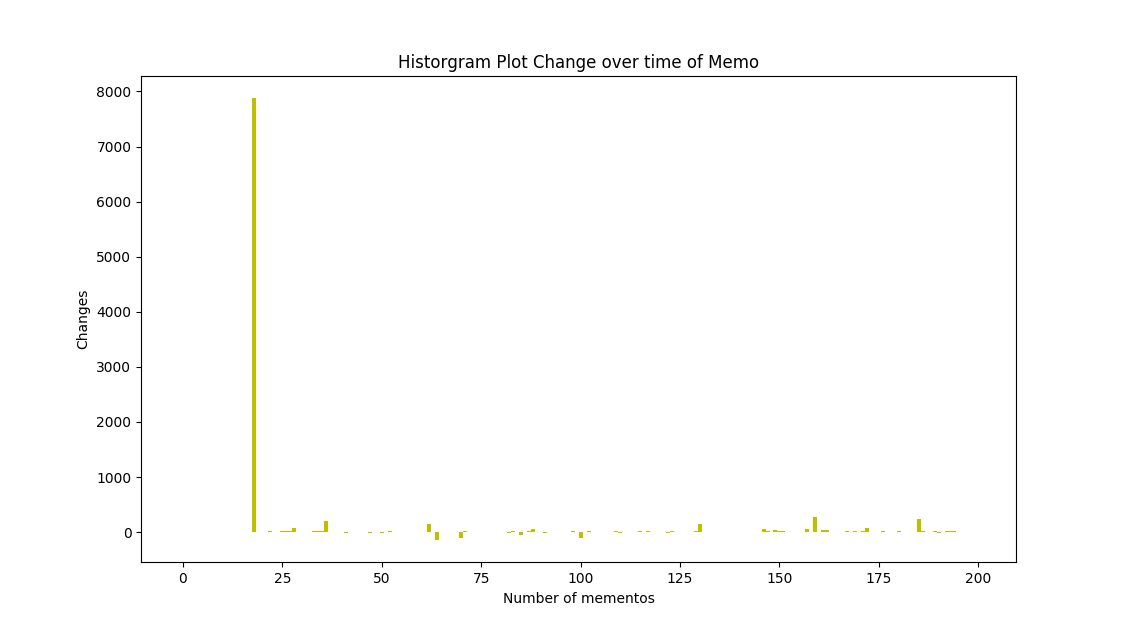
\includegraphics[scale=.3]{Figure_1.png}
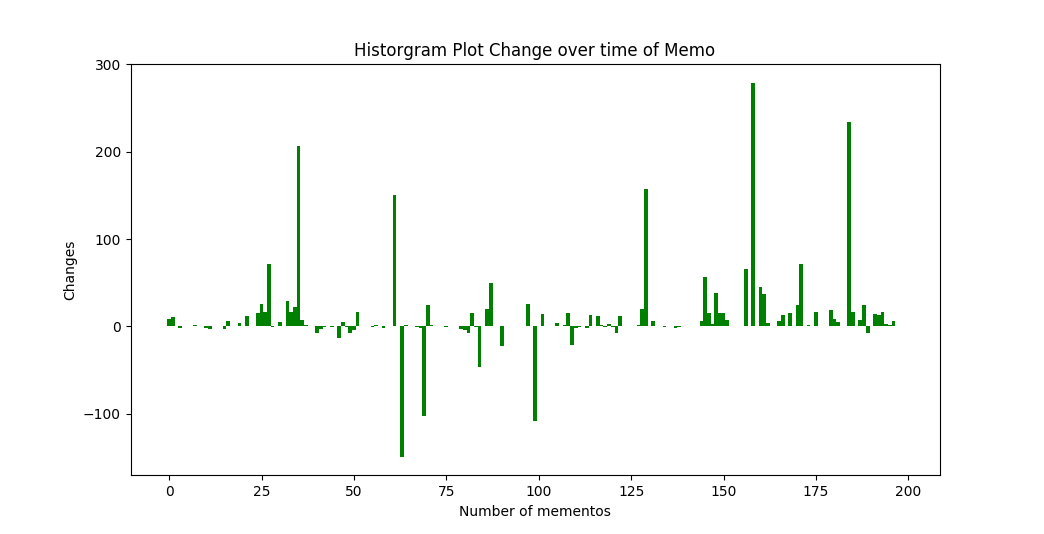
\includegraphics[scale=.4]{Figure_2.png}
\\
\pagebreak
\end{document}